% move all configuration stuff into includes file so we can focus on the content
\documentclass[aspectratio=169,hyperref={pdfpagelabels=false,colorlinks=true,linkcolor=white,urlcolor=lightblue},xcolor={table},t]{beamer}

%%%%%%%%%%%%%%%%%%%%%%%%%%%%%%%%%%%%%%%%%%%%%%%%%%%%%%%%%%%%%%%%%%%%%%%%%%%%%%%%%%
%%%%%%%%%%%%%%%%%%%%%%%%%%%%%%%%%%%%%%%%%%%%%%%%%%%%%%%%%%%%%%%%%%%%%%%%%%%%%%%%%%
% packages
\usepackage{pict2e}
\usepackage{epic}
\usepackage{amsmath,amsfonts,amssymb}
\usepackage{units}
\usepackage{fancybox}
\usepackage[absolute,overlay]{textpos} 
%\usepackage[table]{xcolor}
\usepackage{animate}
\usepackage{gensymb}
%\usepackage{graphicx}
%\usepackage{longtable}
\usepackage{multirow}
\usepackage{silence}
\usepackage{tikz}
\usepackage[backend=bibtex,style=ieee]{biblatex}
\AtEveryCitekey{\iffootnote{\tiny}{}}
\addbibresource{include/references}



% fontsize
\let\Tiny=\tiny

%%%%%%%%%%%%%%%%%%%%%%%%%%%%%%%%%%%%%%%%%%%%%%%%%%%%%%%%%%%%%%%%%%%%%%%%%%%%%%%%%%
%%%%%%%%%%%%%%%%%%%%%%%%%%%%%%%%%%%%%%%%%%%%%%%%%%%%%%%%%%%%%%%%%%%%%%%%%%%%%%%%%%
% warnings
\pdfsuppresswarningpagegroup=1
\WarningFilter{biblatex}{Patching footnotes failed}
\WarningFilter{latexfont}{Font shape}
\WarningFilter{latexfont}{Some font shapes}
\WarningFilter{gensymb}{Not defining}


%%%%%%%%%%%%%%%%%%%%%%%%%%%%%%%%%%%%%%%%%%%%%%%%%%%%%%%%%%%%%%%%%%%%%%%%%%%%%%%%%%
%%%%%%%%%%%%%%%%%%%%%%%%%%%%%%%%%%%%%%%%%%%%%%%%%%%%%%%%%%%%%%%%%%%%%%%%%%%%%%%%%%
% theme & layout
\usetheme{Frankfurt}
\useinnertheme{rectangles}


%%%%%%%%%%%%%%%%%%%%%%%%%%%%%%%%%%%%%%%%%%%%%%%%%%%%%%%%%%%%%%%%%%%%%%%%%%%%%%%%%%
\setbeamertemplate{frametitle}[default][colsep=-4bp,rounded=false,shadow=false]
\setbeamertemplate{frametitle}
{%
    \nointerlineskip%
    %\vskip-0.5ex
    \begin{beamercolorbox}[wd=\paperwidth,ht=3.5ex,dp=0.6ex]{frametitle}
        \hspace*{1.3ex}\insertframetitle%
        
        \hspace*{1.3ex}\small\insertframesubtitle%
    \end{beamercolorbox}%
    \begin{textblock*}{100mm}(13.75cm,1cm)
        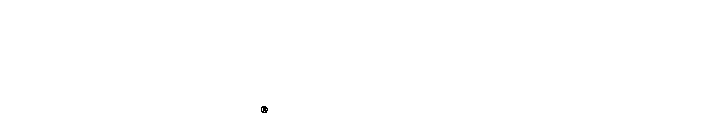
\includegraphics[height=.4cm,keepaspectratio]{graph/Logo_GTCMT_white}
    \end{textblock*}
}


%%%%%%%%%%%%%%%%%%%%%%%%%%%%%%%%%%%%%%%%%%%%%%%%%%%%%%%%%%%%%%%%%%%%%%%%%%%%%%%%%%
\setbeamertemplate{title page}[default][colsep=-4bp,rounded=false,shadow=false]
\setbeamertemplate{title page}
{
    \begin{textblock*}{100mm}(15cm,.51cm)
            \href{https://github.com/alexanderlerch/ACA-Slides/blob/2nd_edition/\jobname.pdf}{\includegraphics[height=.5cm,keepaspectratio]{graph/Logo_github}}\hspace*{2ex}
    \end{textblock*}
    \begin{textblock*}{100mm}(15cm,1.3cm)
            \href{\IEEELink}{
\includegraphics[height=.5cm,keepaspectratio]{graph/icon/book}}\hspace*{2ex}
    \end{textblock*}
    \vskip-10ex
    \begin{beamercolorbox}[wd=\paperwidth,ht=.7\paperheight,dp=0.6ex]{frametitle} %35ex
        %\begin{flushright}
            %\href{http://www.gtcmt.gatech.edu}{
\includegraphics[height=.8cm,keepaspectratio]{graph/Logo_GTCMT_black}}\hspace*{2ex}
        %\end{flushright}
        
        \hspace*{1.8ex}\LARGE\inserttitle%
        
        \vspace*{.5ex}
        
        \hspace*{1.3ex}\small\insertsubtitle%
        
        \vspace*{.5ex}
    \end{beamercolorbox}%
    \nointerlineskip%
    \begin{beamercolorbox}[wd=\paperwidth,ht=.4\paperheight,dp=0.6ex]{page number in head/foot}
        %\vspace*{-.5ex}
        \hspace*{1.7ex}\small\insertauthor%
        
        %\hspace*{1.7ex}\small }%
        
        \vspace*{12ex}
        \vfill
        \begin{flushright}
            \href{http://www.gtcmt.gatech.edu}{
\includegraphics[height=.5cm,keepaspectratio]{graph/Logo_GTCMT_black}}\hspace*{2ex}
        \end{flushright}
    \end{beamercolorbox}%
}


%%%%%%%%%%%%%%%%%%%%%%%%%%%%%%%%%%%%%%%%%%%%%%%%%%%%%%%%%%%%%%%%%%%%%%%%%%%%%%%%%%
%\makeatother
\setbeamertemplate{footline}
{
  \leavevmode%
  \hbox{%
  \begin{beamercolorbox}[wd=.5\paperwidth,ht=2.25ex,dp=1ex,left,leftskip=1ex]{page number in head/foot}%
    \insertsubtitle
  \end{beamercolorbox}%
  \begin{beamercolorbox}[wd=.5\paperwidth,ht=2.25ex,dp=1ex,right,rightskip=1ex]{page number in head/foot}%
    \hfill
    \insertframenumber{} / \inserttotalframenumber
  \end{beamercolorbox}}%
  \vskip0pt%
}
%\makeatletter


%%%%%%%%%%%%%%%%%%%%%%%%%%%%%%%%%%%%%%%%%%%%%%%%%%%%%%%%%%%%%%%%%%%%%%%%%%%%%%%%%%
\beamertemplatenavigationsymbolsempty
\setbeamertemplate{navigation symbols}{}
\setbeamertemplate{blocks}[default]%[rounded=false,shadow=false]
\setbeamertemplate{itemize item}[square]
\setbeamertemplate{itemize subitem}[circle]
\setbeamertemplate{itemize subsubitem}[triangle]
\setbeamertemplate{enumerate item}[square]
\setbeamertemplate{enumerate subitem}[circle]
\setbeamertemplate{enumerate subsubitem}[circle]


%%%%%%%%%%%%%%%%%%%%%%%%%%%%%%%%%%%%%%%%%%%%%%%%%%%%%%%%%%%%%%%%%%%%%%%%%%%%%%%%%%
% colors
\setbeamercolor{structure}{fg=darkgray}
\setbeamercovered{transparent} %invisible
\setbeamercolor{bibliography entry author}{fg=black}
\setbeamercolor*{bibliography entry title}{fg=black}
\setbeamercolor*{bibliography entry note}{fg=black}
\setbeamercolor{frametitle}{fg=black}
\setbeamercolor{title}{fg=white}
\setbeamercolor{subtitle}{fg=white}
\setbeamercolor{frametitle}{fg=white}
\setbeamercolor{framesubtitle}{fg=white}
\setbeamercolor{mini frame}{fg=white, bg=black}
\setbeamercolor{section in head/foot}{fg=white, bg=darkgray}
\setbeamercolor{page number in head/foot}{fg=black, bg=lightblue}
\setbeamercolor{item projected}{fg=white, bg=black}

%---------------------------------------------------------------------------------
%%%%%%%%%%%%%%%%%%%%%%%%%%%%%%%%%%%%%%%%%%%%%%%%%%%%%%%%%%%%%%%%%%%%%%%%%%%%%%%%%%
%%%%%%%%%%%%%%%%%%%%%%%%%%%%%%%%%%%%%%%%%%%%%%%%%%%%%%%%%%%%%%%%%%%%%%%%%%%%%%%%%%
% title information
\title[]{Introduction to \textbf{Audio Content Analysis}}   
\author[alexander lerch]{alexander lerch} 
%\institute{~}
%\date[Alexander Lerch]{}
%\titlegraphic{\vspace{-16mm}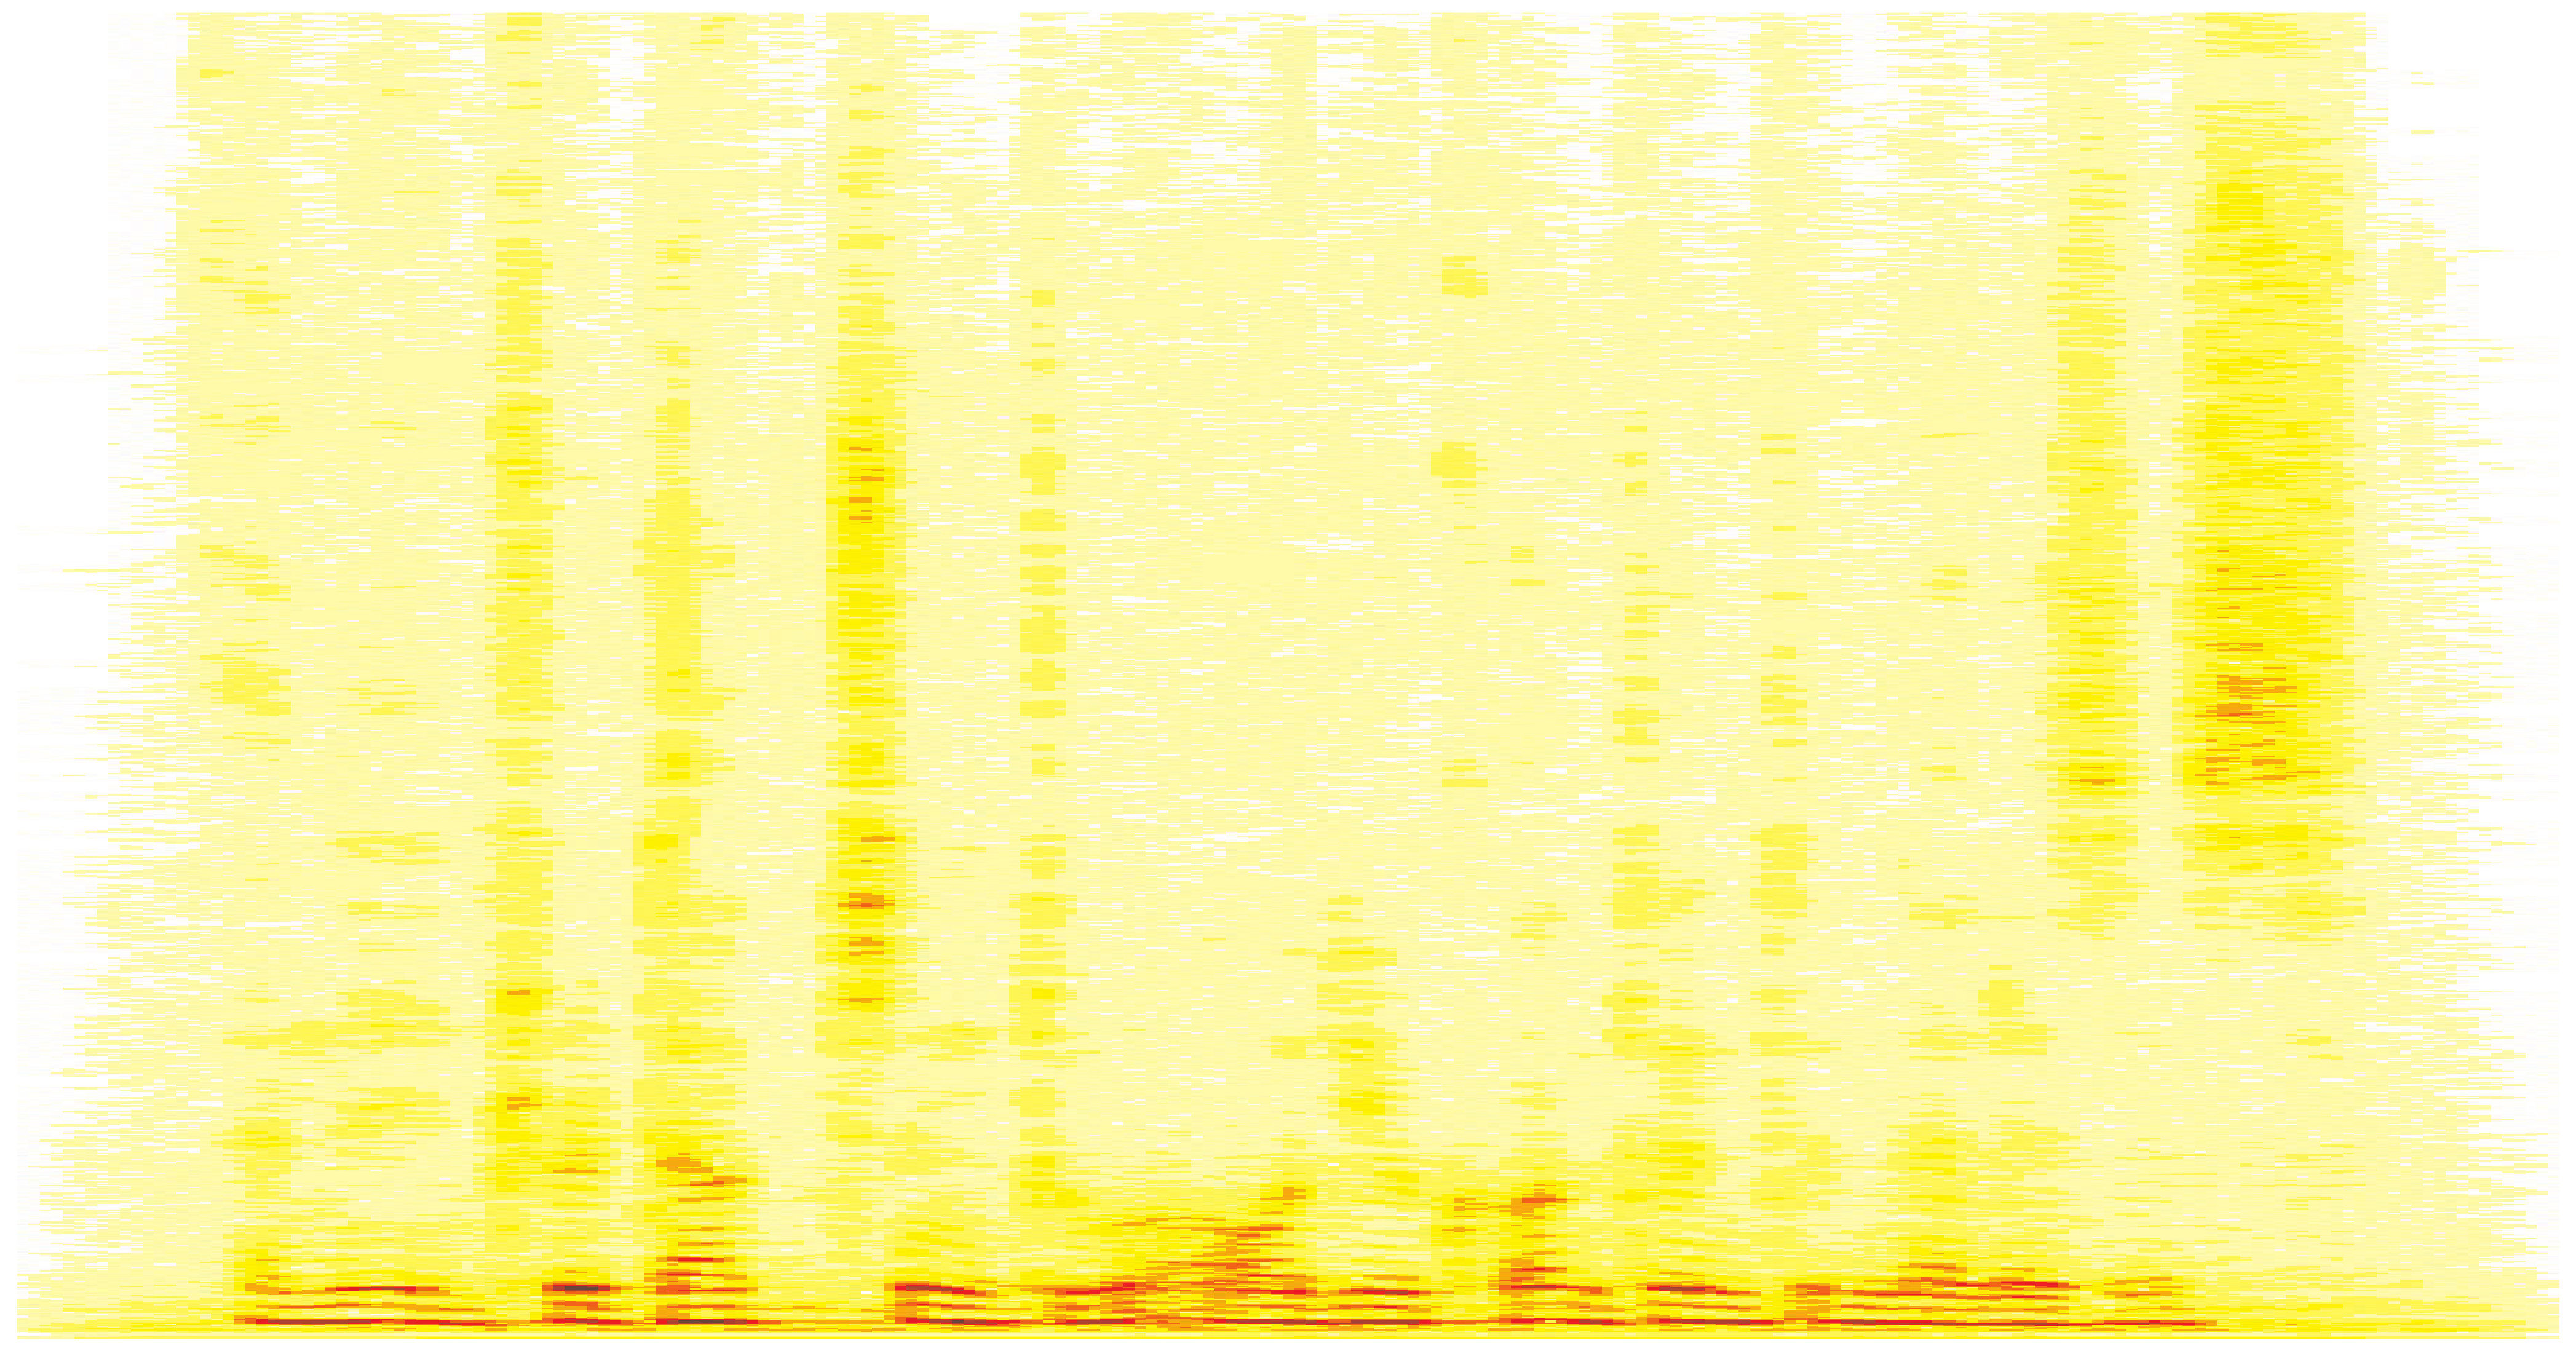
\includegraphics[width=\textwidth,height=3cm]{title}}

%%%%%%%%%%%%%%%%%%%%%%%%%%%%%%%%%%%%%%%%%%%%%%%%%%%%%%%%%%%%%%%%%%%%%%%%%%%%%%%%%%
%%%%%%%%%%%%%%%%%%%%%%%%%%%%%%%%%%%%%%%%%%%%%%%%%%%%%%%%%%%%%%%%%%%%%%%%%%%%%%%%%%
% colors
\definecolor{gtgold}{HTML}{96caff} %0e7eed {rgb}{0.88,0.66,1,0.06} [234, 170, 0]/256
\definecolor{darkgray}{rgb}{.1, .1, .25}
\definecolor{lightblue}{HTML}{0e7eed}
\definecolor{highlight}{rgb}{0, 0, 1} %_less!40

%%%%%%%%%%%%%%%%%%%%%%%%%%%%%%%%%%%%%%%%%%%%%%%%%%%%%%%%%%%%%%%%%%%%%%%%%%%%%%%%%%
%%%%%%%%%%%%%%%%%%%%%%%%%%%%%%%%%%%%%%%%%%%%%%%%%%%%%%%%%%%%%%%%%%%%%%%%%%%%%%%%%%
% relative paths
\graphicspath{{../ACA-Plots/graph/}}


%%%%%%%%%%%%%%%%%%%%%%%%%%%%%%%%%%%%%%%%%%%%%%%%%%%%%%%%%%%%%%%%%%%%%%%%%%%%%%%%%%
%%%%%%%%%%%%%%%%%%%%%%%%%%%%%%%%%%%%%%%%%%%%%%%%%%%%%%%%%%%%%%%%%%%%%%%%%%%%%%%%%%
% units
\setlength{\unitlength}{1mm}

%%%%%%%%%%%%%%%%%%%%%%%%%%%%%%%%%%%%%%%%%%%%%%%%%%%%%%%%%%%%%%%%%%%%%%%%%%%%%%%%%%
%%%%%%%%%%%%%%%%%%%%%%%%%%%%%%%%%%%%%%%%%%%%%%%%%%%%%%%%%%%%%%%%%%%%%%%%%%%%%%%%%%
% math
\DeclareMathOperator*{\argmax}{argmax}
\DeclareMathOperator*{\argmin}{argmin}
\DeclareMathOperator*{\atan}{atan}
\DeclareMathOperator*{\arcsinh}{arcsinh}
\DeclareMathOperator*{\sign}{sign}
\DeclareMathOperator*{\tcdf}{tcdf}
\DeclareMathOperator*{\si}{sinc}
\DeclareMathOperator*{\princarg}{princarg}
\DeclareMathOperator*{\arccosh}{arccosh}
\DeclareMathOperator*{\hwr}{HWR}
\DeclareMathOperator*{\flip}{flip}
\DeclareMathOperator*{\sinc}{sinc}
\DeclareMathOperator*{\floor}{floor}
\newcommand{\e}{{e}}
\newcommand{\jom}{\mathrm{j}\omega}
\newcommand{\jOm}{\mathrm{j}\Omega}
\newcommand   {\mat}[1]    		{\boldsymbol{\uppercase{#1}}}		%bold
\renewcommand {\vec}[1]    		{\boldsymbol{\lowercase{#1}}}		%bold

%%%%%%%%%%%%%%%%%%%%%%%%%%%%%%%%%%%%%%%%%%%%%%%%%%%%%%%%%%%%%%%%%%%%%%%%%%%%%%%%%%
%%%%%%%%%%%%%%%%%%%%%%%%%%%%%%%%%%%%%%%%%%%%%%%%%%%%%%%%%%%%%%%%%%%%%%%%%%%%%%%%%%
% media9
\newcommand{\includeaudio}[1]{
\href{run:audio/#1.mp3}{
\includegraphics[width=5mm, height=5mm]{graph/SpeakerIcon}}}

\newcommand{\includeanimation}[4]{{\begin{center}
                        \animategraphics[autoplay,loop,scale=.7]{#4}{animation/#1-}{#2}{#3}        
                        \end{center}
                        \addreference{matlab source: \href{https://github.com/alexanderlerch/ACA-Plots/blob/master/matlab/animate#1.m}{matlab/animate#1.m}}}
                        \inserticon{video}}
                        
%%%%%%%%%%%%%%%%%%%%%%%%%%%%%%%%%%%%%%%%%%%%%%%%%%%%%%%%%%%%%%%%%%%%%%%%%%%%%%%%%%
%%%%%%%%%%%%%%%%%%%%%%%%%%%%%%%%%%%%%%%%%%%%%%%%%%%%%%%%%%%%%%%%%%%%%%%%%%%%%%%%%%
% other commands
\newcommand{\question}[1]{%\vspace{-4mm}
                          \setbeamercovered{invisible}
                          \begin{columns}[T]
                            \column{.9\textwidth}
                                \textbf{#1}
                            \column{.1\textwidth}
                                \vspace{-8mm}
                                \begin{flushright}
                                     
\includegraphics[width=.9\columnwidth]{graph/question_mark}
                                \end{flushright}
                                \vspace{6mm}
                          \end{columns}\pause\vspace{-12mm}}

\newcommand{\toremember}[1]{
                        \inserticon{lightbulb}
                        }

\newcommand{\matlabexercise}[1]{%\vspace{-4mm}
                          \setbeamercovered{invisible}
                          \begin{columns}[T]
                            \column{.8\textwidth}
                                \textbf{matlab exercise}: #1
                            \column{.2\textwidth}
                                \begin{flushright}
                                     
\includegraphics[scale=.5]{graph/logo_matlab}
                                \end{flushright}
                                %\vspace{6mm}
                          \end{columns}}

\newcommand{\addreference}[1]{  
                  
                    \begin{textblock*}{\baselineskip }(.98\paperwidth,.5\textheight) %(1.15\textwidth,.4\textheight)
                         \begin{minipage}[b][.5\paperheight][b]{1cm}%
                            \vfill%
                             \rotatebox{90}{\tiny {#1}}
                        \end{minipage}
                   \end{textblock*}
                    }
                    
\newcommand{\figwithmatlab}[1]{
                    \begin{figure}
                        \centering
                        \includegraphics[scale=.7]{#1}
                        %\label{fig:#1}
                    \end{figure}
                    
                    \addreference{matlab source: \href{https://github.com/alexanderlerch/ACA-Plots/blob/main/matlab/plot#1.m}{plot#1.m}}}
\newcommand{\figwithref}[2]{
                    \begin{figure}
                        \centering
                        \includegraphics[scale=.7]{#1}
                        \label{fig:#1}
                    \end{figure}
                    
                    \addreference{#2}}  
                                    
\newcommand{\inserticon}[1]{
                    \begin{textblock*}{100mm}(14.5cm,7.5cm)
                        \includegraphics[height=.8cm,keepaspectratio]{graph/#1}
                    \end{textblock*}}            

%%%%%%%%%%%%%%%%%%%%%%%%%%%%%%%%%%%%%%%%%%%%%%%%%%%%%%%%%%%%%%%%%%%%%%%%%%%%%%%%%%
%%%%%%%%%%%%%%%%%%%%%%%%%%%%%%%%%%%%%%%%%%%%%%%%%%%%%%%%%%%%%%%%%%%%%%%%%%%%%%%%%%
% counters
\newcounter{i}
\newcounter{j}
\newcounter{iXOffset}
\newcounter{iYOffset}
\newcounter{iXBlockSize}
\newcounter{iYBlockSize}
\newcounter{iYBlockSizeDiv2}
\newcounter{iXBlockSizeDiv2}
\newcounter{iDistance}

\newcommand{\IEEELink}{https://ieeexplore.ieee.org/servlet/opac?bknumber=9965970}




\subtitle{module 9.1: introduction to tempo \& rhythm terminology}

%%%%%%%%%%%%%%%%%%%%%%%%%%%%%%%%%%%%%%%%%%%%%%%%%%%%%%%%%%%%%%%%%%%%%%%%%%%%
\begin{document}
    % generate title page
	{
\setbeamertemplate{headline}{} 
\setbeamertemplate{footline}{} 
\begin{frame}
    \titlepage
    %\vspace{-5mm}
\end{frame}
}
\addtocounter{framenumber}{-1}


    \section[overview]{lecture overview}
        \begin{frame}{introduction}{overview}
            \begin{block}{corresponding textbook section}
                    %\href{http://ieeexplore.ieee.org/xpl/articleDetails.jsp?arnumber=6331123}{Chapter 6~---~Temporal Analysis}: pp.~129--135
                    sections~9.1 \& 9.2
            \end{block}

            \begin{itemize}
                \item   \textbf{lecture content}
                    \begin{itemize}
                        \item   terminology for rhythm detection
                        \item   perceptually motivated rhythm accuracy
                    \end{itemize}
                \bigskip
                \item<2->   \textbf{learning objectives}
                    \begin{itemize}
                        \item   describe the terms onset, tempo, meter, bar, and rhythm
                        \item   give two examples of typical onset times for musical instruments
                    \end{itemize}
            \end{itemize}
            \inserticon{directions}
        \end{frame}

    \section[intro]{introduction}
        \begin{frame}{temporal events}{introduction}
            \begin{itemize}
                \item  \textbf{categorization of temporal parameters}:
                    \begin{itemize}
                        \item	\textit{score} parameters:\\ structure, time signature, rhythm, \ldots
                        \item	\textit{performance} parameters:\\ tempo, timing, \ldots
                    \end{itemize}
                \bigskip
                \item<2->   \textbf{perception of temporal parameters}:
                    \begin{itemize}
                        \item	audio signal/stream is segmented into distinct events $\Rightarrow$ \textit{onsets} (segment start)
                        \item	humans \textit{structure and group} these events due to position, salience, \ldots
                    \end{itemize}
            \end{itemize}
        \end{frame}

    \section[perception]{human perception of temporal events}
        \begin{frame}{human perception of temporal events}{introduction to onsets}
            \vspace{-3mm}
            \begin{itemize}
                \item   \textbf{onset} is start of a musical event
                \smallskip
                \item<1->   \textbf{properties}:
                    \begin{itemize}
                        \item<1->	position
                        \item<1->	strength, salience
                        \item<1->	length?
                    \end{itemize}
            \end{itemize}
                \vspace{-3mm}
                {\figwithmatlab{Onset}}
        \end{frame}

        \begin{frame}{human perception of temporal events}{initial transients}
            \begin{columns}
                \column{.4\linewidth}
                \begin{itemize}
                    \item	percussive instruments:
                    \begin{itemize}
                        \item   \unit[3-20]{ms}
                    \end{itemize}
                    \smallskip
                    \item	woodwind instruments:
                    \begin{itemize}
                        \item   up to \unit[300]{ms}
                    \end{itemize}
                    \bigskip
                    \item<2->	typical range for majority of instruments:
                    \begin{itemize}
                        \item   \unit[15--50]{ms}
                    \end{itemize}
                \end{itemize}
                \column{.6\linewidth}
                \begin{figure}
                \includegraphics[width=\columnwidth]{Onset}
                \end{figure}            
            \end{columns}
        \end{frame}
        \begin{frame}{human perception of temporal events}{human detection accuracy}
            \vspace{-3mm}
            \begin{itemize}
                \item	\textit{detection \& discrimination} of 2 subsequent onsets
                    \begin{itemize}
                        \item	detection $\Delta t > \unit[2]{ms}$, discrimination $\Delta t > \unit[20]{ms}$\only<1>{\footfullcite{hirsh_auditory_1959}}
                    \end{itemize}
                
                \smallskip
                \item<2->	\textit{prediction} of looped monophonic instrument onsets
                    \begin{itemize}
                        \item	IOI \unit[600]{ms}: $\sigma = \unit[12]{ms}$\only<2>{\footfullcite{gordon_perception_1984}}
                        \item	IOI $<$ \unit[240]{ms}: $\sigma = \unit[10]{ms}$\only<2>{\footfullcite{friberg_perception_1992}}
                    \end{itemize}

                \smallskip
                \item<3->	manual onset time \textit{annotation}
                    \begin{itemize}
                        \item	piano: mean abs.\ error: \unit[4.3]{ms}, max: \unit[35]{ms}\only<3>{\footfullcite{repp_diversity_1992}}
                        \item	various: mean abs.\ error: \unit[10]{ms}, max: \unit[30]{ms}\only<3>{\footfullcite{leveau_methodology_2004}}
                    \end{itemize}
                
                \smallskip
                \item<4->	ensemble performance
                    \begin{itemize}
                        \item	string \& woodwind: deviations up to  \unit[30-50]{ms}\only<4>{\footfullcite{rasch_synchronization_1979}}
                        \item	piano: $\sigma = \unit[14-38]{ms}$\only<4>{\footfullcite{shaffer_timing_1984}}
                    \end{itemize}
            \end{itemize}
        \end{frame}

        \begin{frame}{human perception of temporal events}{offsets}
            \question{what about offsets/end of notes}

            \begin{itemize}
                \item   \textbf{perceptually not as important} as an onset
                    \begin{itemize}
                        \item   offset are often ignored in rhythm perception
                    \end{itemize}
                \smallskip
                \item	\textbf{systematic difficulties}: when does a note end?
                    \begin{itemize}
                        \item	performer stops excitation
                        \item	instrument stops oscillation
                        \item	listener cannot recognize it anymore
                    \end{itemize}
                \smallskip
                \item	\textbf{practical difficulties}: hard to detect
                    \begin{itemize}
                        \item	low volume
                        \item	reverberation
                        \item	masking
                    \end{itemize}
            \end{itemize}
        \end{frame}
        
        \begin{frame}{human perception of temporal events}{tempo, meter \& rhythm}
            \vspace{-2mm}
            \begin{itemize}
                \item	\textbf{tempo}: perceived equal duration pulses at a ``natural'' rate~---~tactus
                    \begin{itemize}
                        
                        \item<1->	constant tempo
                            \begin{footnotesize}
                            \begin{equation*}\label{eq:tempo_mean}
                                \mathfrak{T} = \frac{ \mathcal{B}\cdot \unit[60]{s}}{\Delta t_\mathrm{s}}\;\; [\unit{BPM}] 
                            \end{equation*}
                            \end{footnotesize}
                        \item<1->	dynamic tempo
                            \begin{footnotesize}
                            \begin{equation*}
                                \mathfrak{T}_\mathrm{local}(j) = \frac{\unit[60]{s}}{t_\mathrm{b}(j+1)-t_\mathrm{b}(j)}\;\; [\unit{BPM}] 
                            \end{equation*}
                            \end{footnotesize}
                            
                            
                        \item    perceived overall tempo?
                            \begin{itemize}
                                \item	average, main, mode, \ldots
                            \end{itemize}
                    \end{itemize}
                \smallskip                
                \item<2->	\textbf{meter}
                    \begin{itemize}
                        \item	group of strong and weak musical elements/beats
                        
                        \item	typically 3 to 7 beats (app.\ \unit[5]{s})
                    \end{itemize}
                
                \smallskip                
                \item<3->	\textbf{rhythm}
                    \begin{itemize}
                        \item	group length \unit[1--8]{beats}
                        \item	defined by accents and time intervals
                    \end{itemize}
            \end{itemize}
        \end{frame}
        
        \begin{frame}{temporal events}{hierarchical structure}
            \figwithmatlab{BeatHierarchy}
        \end{frame}

    \section[musical]{musical notation of temporal events}
        \begin{frame}{musical notation of temporal events}{tempo, time signature, bar \& note value}
            \begin{itemize}
                \item	\textbf{tempo}
                    \begin{itemize}
                        \item	\textsl{Largo}, \textsl{Adagio}, \textsl{Andante}, \textsl{Moderato}, \textsl{Allegro}, \textsl{Presto}
                        \item	\textsl{ritardando}, \textsl{accelerando}, \ldots
                        \item	modern scores: sometimes overall tempo in \unit{BPM}
                    \end{itemize}
                \smallskip
                \item<1->	\textbf{bar}
                    \begin{itemize}
                        \item	score equivalent of perceptual meter
                        \item	begin of bar is marked by a vertical line
                    \end{itemize}
                \smallskip
                \item<1->	\textbf{time signature}
                    \begin{itemize}
                        \item	conveys length of bar
                            \only<1->{\begin{flushright}
                                \vspace{-10mm}
                                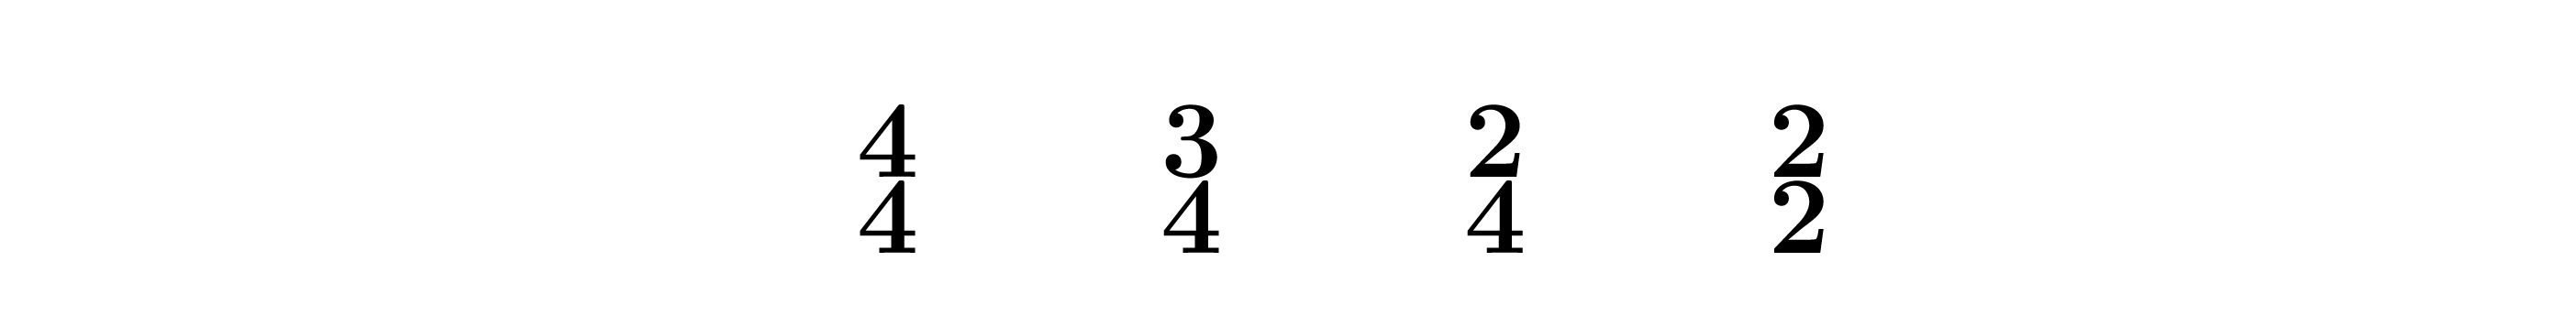
\includegraphics[scale=.5]{graph/onset_timesigs}
                            \end{flushright}}
                    \end{itemize}
                \smallskip
                \item<1->	\textbf{note value}
                            \only<1->{\begin{flushright}
                                \vspace{-5mm}
                                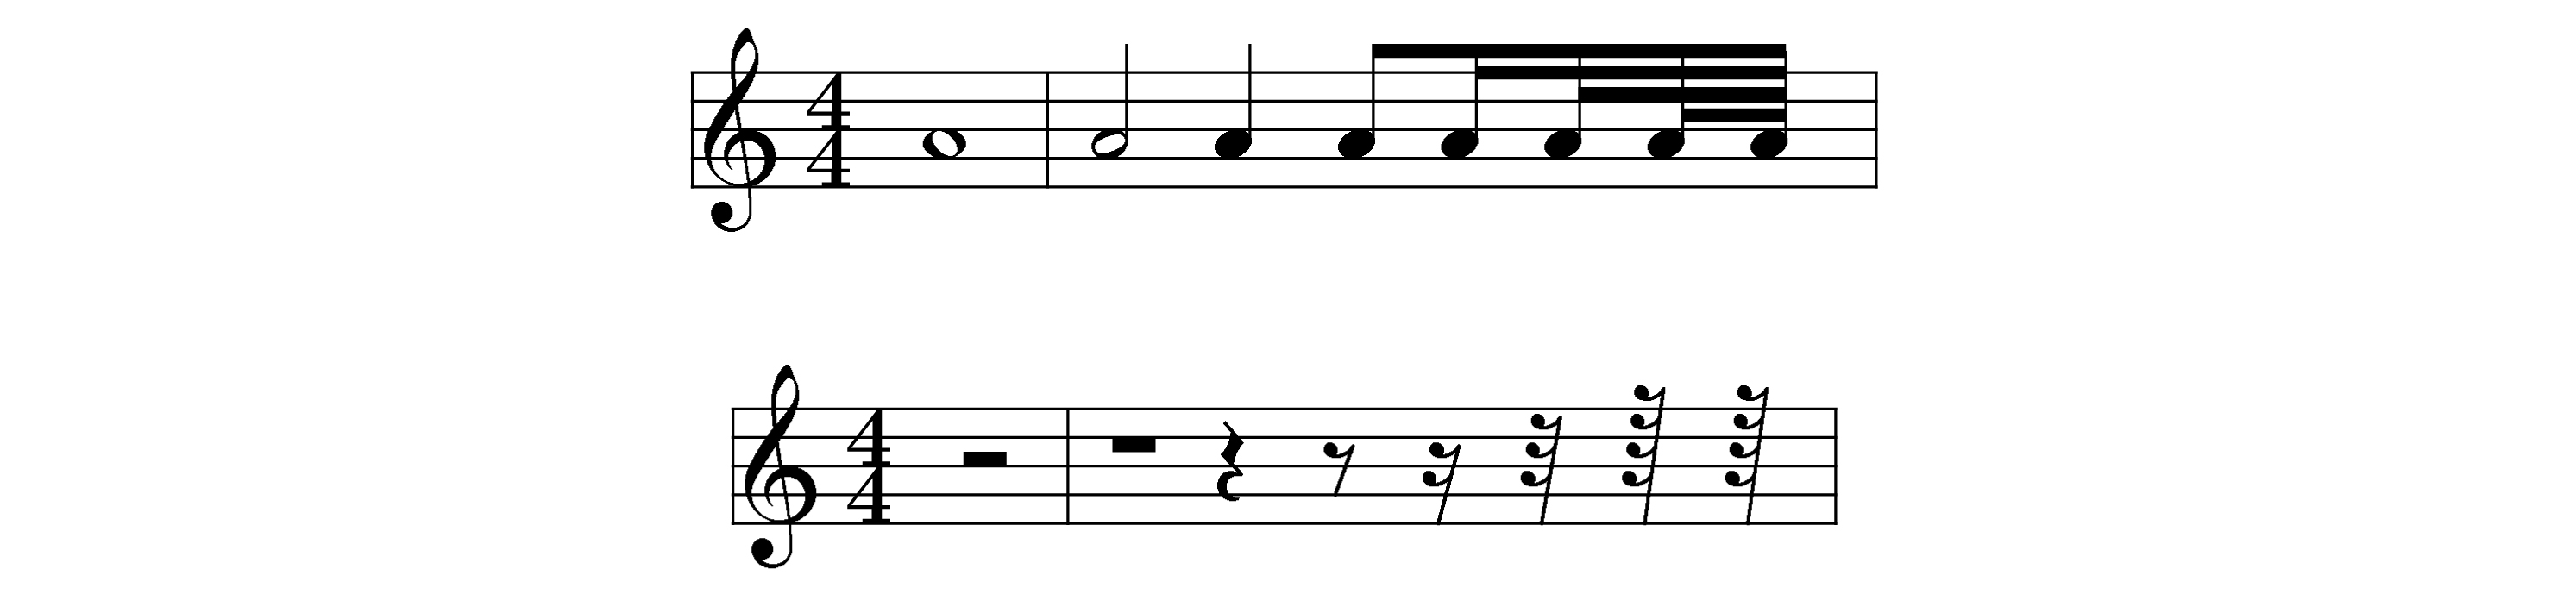
\includegraphics[scale=.6]{graph/onset_notevalues}
                            \end{flushright}}
            \end{itemize}
        \end{frame}
    
    \section{summary}
        \begin{frame}{summary}{lecture content}
            \begin{itemize}
                \item   \textbf{perceptual terms}
                    \begin{itemize}
                        \item   onset, tempo, meter, rhythm
                    \end{itemize}
                \bigskip
                \item   \textbf{musical terms}
                    \begin{itemize}
                        \item   tempo, bar, time signature, note value, rhythm
                    \end{itemize}
                \bigskip
                \item   \textbf{accuracy range of interest}
                    \begin{itemize}
                        \item   \unit[2--300]{ms}
                    \end{itemize}
            \end{itemize}
            
            \inserticon{summary}
        \end{frame}
\end{document}
